\documentclass[a4paper,norsk]{article}
\usepackage{preamble}
\usepackage{tabu}
\usepackage{color, colortbl}
\definecolor{LightCyan}{rgb}{0.88,1,1}

\begin{document}
\maketitle
We let $((x_k, y_k, z_k))_{k=1}^m$ be some available data points in $\mathbb{R}^3$, and we want to define a model based on a smaller set of 
coordinates ${(u_j, v_j)}_{j=1}^n$ in $\mathbb{R}^2$. As mentioned in the introduction $(u_j, v_j)$ will be the vertices of the triangles yodelling the the set of
data points. Further we define piecewise linear functions ${N_j(x, y)}_{j=1}^n$ such that $N_j(u_j, v_j) = 1$, $N_j(u_i, v_i) = 0$ if i $\neq$ j. These functions are much alike the "hat functions" found in the Finite Element method. Our goal will be to find a least squares fit to approximate the given dataset with these functions.

\section*{Exercise 1}
\begin{figure}[h!]
	\centering
	\caption*{\textbf{Visualisations of a piecewise linear function $N_j$ \newline (Figure from MEK4250 course book)}}
	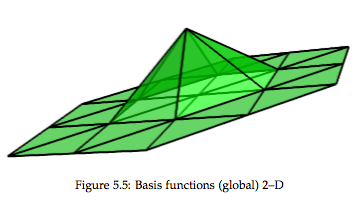
\includegraphics[scale=0.36]{element.png}
\end{figure}

Our set of linear functions ${N_j(x, y)}_{j=1}^n$ are linear independent if \begin{align*}
\sum_{j=1}^n c_j N_j(x,y) = c_1 N_1 + c_2 N_2 .... c_n N_n = 0 
\end{align*}
for the trivial solution $c_1 = c_2 .. c_n = 0$. 
\\Let us assume that at least two ${u_j, v_j}$ are located at the same point, say $j = 1,2$. Then by definition $N_1(u_1, v_1)$ and $N_2(u_2, v_2)$ will be defined over same area with the same properties as introduced. Hence our linear system can be written as 
$\sum_{j=1}^n c_j N_j(x,y) = c_1 N_1 + c_2 N_2 .... c_n N_n = (c_1 + c_2)N_2 + c_3 N_3 .... c_n N_n = 0$. Hence the system has a nontrivial solution, and the set of functions are linear dependent. We therefore must
choose ${(u_j, v_j)}_{j=1}^n$ at different points to have a linear independent set of functions. 

\newpage
\section*{Exercise 2}
For simplicity let  ${(u_j, v_j)}_{j=1}^n$ for n < m, be our chosen coordinates from the dataset such that $(u_1, v_1) = (x_1, y_1), (u_2, v_2) = (x_2, y_2),.., (u_n, v_n) = (x_n, y_n)$ increasing index order. For a linear independent system we must have that that 
\begin{align*}
\sum_{k=1}^n \Big(\sum_{j=1}^n c_j N_j(x_k,y_k) \Big) + \sum_{k=n+1}^m \Big(\sum_{j=1}^n c_j N_j(x_k,y_k) \Big) = 0
\end{align*}
Since
\begin{align*} 
\sum_{k=1}^n \Big(\sum_{j=1}^n c_j N_j(x_k,y_k) \Big)= \sum_{k=1}^n \Big(\sum_{j=1}^n c_j N_j(u_k,v_k) \Big) = 0
\end{align*}
only has the trivial solution $c_1 + c_2 .... c_n  = 0$, this holds for the whole system and $B$ is linarly independent.

\section*{Exercise 3}
Now for some k, the triangles sharing $(u_k, v_k)$ as a vertex spans the function $N_k$. Clearly if these triangles doesn't contain any data point (x_j, y_j), then
$\sum_{j=1}^n N_k(x_j,y_j) = 0$. As a result we have a zero column of $B$, and $\sum_{j=1}^n c_j N_j(x,y) = 0 $ has a non-trivial solution, since $c_k$ can be choosen freely.


\newpage
\section*{Exercise 4}
This simple program writes out the barycentric coordinates of \textbf{p}, relative to the triangle spanned by $\textbf{p}_1$, $\textbf{p}_2$ and $\textbf{p}_3$. 
A simple run set by the coordinates $\textbf{p}_1 = (0, 0)$, $\textbf{p}_2 = (1, 1)$, $\textbf{p}_3 = (-1, 1)$ for $\textbf{p} = (0.5, 0)$ yeilds

\begin{lstlisting}[style=terminal]
Find the barycentric coordinates of (0, 0.5) 
In the triangle spanned by 

p1 = [0, 0]
p2 = [1, 1]
p3 = [-1, 1]

The barycentric coordinates of p relative to the spanned triangle:
b1 = 0.5,  b2 = 0.25,   b3 = 0.25
\end{lstlisting}

\begin{lstlisting}[style=python]
import numpy as np

def barycentric(p1, p2, p3, p):
    #barycentric takes 4 arguments.
    #p1, p2, p3 are the points spanning the triangle, 
    #hence these must not lie on a line
    #p is the point within the triangle

    print "Find the barycentric coordinates of (%g, %g) \n" \
    "In the triangle spanned by \n" % (p[0], p[1])
    count = 1
    for i in [p1, p2, p3]:
        print "p%d = [%g, %g]" % (count, i[0], i[1])
        count += 1

    cond = [1 for i in range(3)]

    #Assemble the left hand side of the system
    A =  np.vstack([p1, p2, p3])
    A = np.append(np.transpose(A), [cond], axis=0)

    #Assemble the right hand side of the system
    L = np.insert(np.array(p), len(p), 1)

    #solve system
    b = np.linalg.solve(A, L)

    #Print result
    print "\nThe barycentric coordinates of p relative to the spanned triangle:"
    print "b1 = %g,  b2 = %g,   b3 = %g" % (b[0], b[1], b[2])

p1 = [0, 0]
p2 = [1, 1]
p3 = [-1, 1]

p = [0, 0.5]

barycentric(p1, p2, p3, p)
\end{lstlisting}

\newpage


\end{document}
